% !TEX program = xelatex

\documentclass[12pt,a4paper]{article}
\usepackage[UTF8]{ctex}
\usepackage{float}
\usepackage{amsmath}
\usepackage{amsfonts}
\usepackage{enumerate}
\usepackage{booktabs}
\usepackage{graphicx}
\usepackage{longtable}
\usepackage{subfigure}

\usepackage{url}
\usepackage{multirow}

% for plotting 
\usepackage{caption}
\usepackage{pgfplots}

% for pseudo code 
\usepackage{algorithm}
\usepackage[noend]{algpseudocode}

% for reference 
\usepackage{hyperref}
\usepackage{cleveref}

% for code 
\usepackage{listings}
\usepackage{xcolor}
\usepackage{fontspec}
\definecolor{darkgreen}{rgb}{0,0.6,0}
\newfontfamily\consolas{Consolas}

\lstset {
    basicstyle=\footnotesize\consolas, % basic font setting
    breaklines=true, 
    frame=single,     % {single, shadowbox, bottomline}
    keywordstyle=\color{blue}, 
    commentstyle=\color{darkgreen},
    stringstyle=\color{red},
    showstringspaces=false,
    % backgroundcolor=\color{black!5}, % set backgroundcolor
    numbers=left, 
    numberstyle=\ttfamily,
}

% Microsoft Word A4 paper default layout 
\usepackage[a4paper, left=3.18cm, right=3.18cm, top=2.54cm, bottom=2.54cm]{geometry}

% \captionsetup[figure]{labelfont={bf}, name={Figure}}
% \captionsetup[table]{labelfont={bf}, name={Table}}

\crefname{equation}{方程}{方程}
\Crefname{equation}{方程}{方程}
\crefname{table}{表}{表}
\Crefname{table}{表}{表}
\crefname{figure}{图}{图}
\Crefname{figure}{图}{图}

\title{数学实验:第六次作业}
\author{计算机系 \quad 计73 \quad 2017011620 \quad 李家昊}
\date{\today}

% 实验报告格式的基本要求

% 系别、班级、学号、姓名

% 1 实验目的
% 2 题目
%   2.1 计算题:题号,算法设计(包括计算公式),程序,计算结果(计算机输出),结果分析,结论。
%   2.2 应用题:题号,问题分析,模型假设,模型建立,算法设计(包括计算公式),程序,计算结果(计算机输出),结果的数学分析,结果的实际意义,结论。
% 3 收获与建议

% Calc
% \subsubsection{算法设计}
% \subsubsection{程序}
% \subsubsection{计算结果}
% \subsubsection{结果分析}
% \subsubsection{结论}

% App
% \subsubsection{问题分析}
% \subsubsection{模型假设}
% \subsubsection{模型建立}
% \subsubsection{算法设计}
% \subsubsection{程序}
% \subsubsection{计算结果}
% \subsubsection{结果的数学分析}
% \subsubsection{结果的实际意义}
% \subsubsection{结论}

\begin{document}

\maketitle

\section{实验目的}

\begin{itemize}
    \item 掌握用MATLAB优化工具箱和LINGO解线性规划的方法。
    \item 练习建立实际问题的线性规划模型。
    \item 掌握用MATLAB优化工具箱和LINGO解非线性规划的方法。
    \item 练习建立实际问题的非线性规划模型。
\end{itemize}

\section{问题求解}

\subsection{Chap8-Ex10 污水处理(应用题)}

\subsubsection{问题分析}

题目给出江边的工厂、污水处理站和居民点的地理位置分布,需要根据工厂污水的流量和水污染浓度、处理站的处理系数、江水的原流量和水污染浓度、各段江水的自净系数等参数,求出在江水污染达到国家标准的情况下,污水处理站的最小总处理费用,这是一个线性规划问题。

\subsubsection{模型假设}

为了简化实际情况,模型基于以下假设,
\begin{enumerate}
    \item 工厂是江水的唯一污染源。
    \item 污水处理站处理前后,水流量不变。
    \item 污水处理站能够将污水净化到所需的任意程度。
    \item 污水与江水能在极短时间内混合均匀。
\end{enumerate}

\subsubsection{模型建立}

设江边共有$n$个工厂,第$1$个工厂位于最上游,第$n$个工厂位于最下游,每个工厂的排污口处设有一个污水处理站,处理站的对岸是一个居民区。对于第$i\ (i=1,2,\cdots,n)$个工厂,记其污水流量为$A_i$,污水浓度为$a_i$,处理站的处理系数为$c_i$,降低的污水浓度为$x_i$,处理站上游的污水流量为$U_i$,浓度为$u_i$,下游的污水流量为$D_i$,浓度为$d_i$,第$i$个到第$i+1$个工厂之间的江水自净系数为$s_i$,国家标准规定的水污染浓度为$r$。其中$A_i,a_i,c_i,s_i\ (i=1,2,\cdots,n)$和$U_1,u_1,r$为已知常数。

需要优化的目标函数为总处理费用,即,
\begin{equation}\label{eq:ex10_target}
    \min f = \sum_{i=1}^n c_i A_i x_i
\end{equation}

决策变量为处理站降低的污水浓度$x_1, x_2, \cdots, x_n$,需要满足取值范围约束,
\begin{equation}\label{eq:ex10_cons_range}
    0 \le x_i \le a_i, \quad i = 1,2,\cdots,n
\end{equation}

第1个工厂的上游水流量$U_1$和污水浓度$u_1$为已知,其余各工厂的上游水流量$U_i$和污水浓度$u_i$满足,
\begin{equation}
    U_i = D_{i-1}, \quad u_i = s_{i-1} d_{i-1}, \quad i = 2,3,\cdots,n
\end{equation}

各工厂的下游水流量$D_i$和污水浓度$d_i$满足,
\begin{equation}
    D_i = U_i + A_i, \quad d_i = \frac{U_i u_i + A_i (a_i - x_i)}{U_i + A_i}, \quad i = 1,2,\cdots,n
\end{equation}

对于第(1)问,需要使江面上所有地段的水污染达到国家标准,则有,
\begin{equation}\label{eq:ex10_cons_updown}
    u_i \le r, \quad d_i \le r, \quad i =1,2,\cdots,n
\end{equation}

对于第(2)问,只要求居民点上游的水污染达到国家标准,则有,
\begin{equation}\label{eq:ex10_cons_up}
    u_i \le r, \quad i =1,2,\cdots,n
\end{equation}

这是一个有约束优化问题,目标函数为\Cref{eq:ex10_target},决策变量为$x_1,x_2,\cdots,x_n$,第(1)问约束条件为\Cref{eq:ex10_cons_range}和\Cref{eq:ex10_cons_updown},第(2)问约束条件为\Cref{eq:ex10_cons_range}和\Cref{eq:ex10_cons_up}。由于目标函数和约束条件均为关于决策变量的线性表示,因此该模型也是一个线性规划模型。

\subsubsection{算法设计}

根据上述分析可知,这是一个线性规划问题,可利用单纯形法求解,对应的MATLAB命令为\texttt{linprog},也可利用LINGO软件求解。

\subsubsection{MATLAB和LINGO程序}

编写了MATLAB版本和LINGO版本的程序,请参见附录\ref{sec:ex10_code}。

\subsubsection{计算结果}

经过实验,MATLAB与LINGO的计算结果完全一致,由于LINGO的分析功能更加强大,因此这里主要叙述LINGO的计算结果。

\paragraph{第(1)问} 令江面上所有地段的水污染均达到国家标准,LINGO经过1次迭代计算得出,总处理费用$f$的最小值为489.50万元,各污水处理站净化的污水浓度$x_1,x_2,x_3$的计算结果如\Cref{tab:ex10_result_updown}所示,江面各处的水质约束情况如\Cref{tab:ex10_result_cons_updown}所示。

\begin{table}[H]
    \centering
    \caption{第(1)问各决策变量的最优值和减少费用}
    \label{tab:ex10_result_updown}
    \begin{tabular}{c|ccc}
        \toprule
        决策变量 & \(x_1\) & \(x_2\) & \(x_3\)\tabularnewline
        \midrule
        最优值 & 59.00 & 38.90 & 0.00\tabularnewline
        减少费用 & 0.00 & 0.00 & 5.00\tabularnewline
        \bottomrule
    \end{tabular}
\end{table}

\begin{table}[H]
    \centering
    \caption{第(1)问各水质约束的松弛变量和对偶价格}
    \label{tab:ex10_result_cons_updown}
    \begin{tabular}{c|cccccc}
        \toprule
        约束条件 & \(u_1\le r\) & \(u_2\le r\) & \(u_3 \le r\) & \(d_1 \le r\) &
        \(d_2 \le r\) & \(d_3 \le r\)\tabularnewline
        \midrule
        松弛变量 & 0.20 & 0.10 & 0.40 & 0.00 & 0.00 & 0.16\tabularnewline
        对偶价格 & 0.00 & 0.00 & 0.00 & 100.50 & 1010.00 & 0.00\tabularnewline
        \bottomrule
    \end{tabular}
\end{table}

\paragraph{第(2)问} 只要求居民点上游的水污染达到国家标准,LINGO经过0次迭代计算得出,总处理费用$f$的最小值为183.33万元,各污水处理站净化的污水浓度$x_1,x_2,x_3$的计算结果如\Cref{tab:ex10_result_up}所示,江面各处的水质约束情况如\Cref{tab:ex10_result_cons_up}所示。

\begin{table}[H]
    \centering
    \caption{第(2)问各决策变量的最优值和减少费用}
    \label{tab:ex10_result_up}
    \begin{tabular}{c|ccc}
        \toprule
        决策变量 & \(x_1\) & \(x_2\) & \(x_3\)\tabularnewline
        \midrule
        最优值 & 36.67 & 0.00 & 0.00\tabularnewline
        减少费用 & 0.00 & 5.00 & 5.00\tabularnewline
        \bottomrule
    \end{tabular}
\end{table}

\begin{table}[H]
    \centering
    \caption{第(2)问各水质约束的松弛变量和对偶价格}
    \label{tab:ex10_result_cons_up}
    \begin{tabular}{c|ccc}
        \toprule
        约束条件 & \(u_1\le r\) & \(u_2\le r\) & \(u_3 \le r\)\tabularnewline
        \midrule
        松弛变量 & 0.20 & 0.00 & 0.22\tabularnewline
        对偶价格 & 0.00 & 1116.67 & 0.00\tabularnewline
        \bottomrule
    \end{tabular}
\end{table}

\subsubsection{结果的数学分析}

在第(1)问中,$x_1,x_2$的减少费用为零,为基变量,约束\(d_1 \le r\)和\(d_2 \le r\)的松弛变量为零,起约束作用。

在第(2)问中,$x_1$的减少费用为零,为基变量,约束\(u_2\le r\)的松弛变量为零,起约束作用。由于此时去掉了第(1)问中两个起作用的约束\(d_1 \le r\)和\(d_2 \le r\),因此最优值比第(1)问更优。若想进一步优化最优值,可以提高工厂1到2之间的江水净化能力,即降低$s_1$,使得约束\(u_2\le r\)更容易被满足。

\subsubsection{结果的实际意义}

由计算结果可以看出,仅要求居民点上游的水质满足国家标准时,所花费的处理费用显著减少,原因是该方案充分利用了江水的自净机制,减轻了污水处理厂的处理压力。在实际的城市规划中也有类似的现象,例如自来水厂通常建在河流的上游,而工厂通常建在下游,使得居民能够用到未污染的水,且河流能充分发挥自净作用。

该计算结果具有一定的实际意义,可作为制定污水处理方案的参考。在实际情况下,还需考虑更多的因素,例如工厂污水排放对河流自净能力的破坏,居民点生活污水的排放对河流的污染,居民取水对水流量的影响等等。在该污水处理方案下,实际的水质是否符合国家标准,还需要通过实验来验证。

\subsubsection{结论}

为了使江面上所有地段的水污染达到国家标准,最少需要花费489.50万元;如果只要求三个居民点上游的水污染达到国家标准,最少需要花费183.33万元。

\subsection{Chap9-Ex4 液体混合(应用题)}

\subsubsection{问题分析}

题目设置了一个生产场景,给定所需原料的价格、成分和最大供应量,最终产品的生产流程、成分指标和最大需求量,需要确定最优的生产方案。一般来说,生产以利润为目的,因此只需在给定约束条件下确定最大利润即可,这是一个非线性规划问题。

\subsubsection{模型假设}

\begin{enumerate}
    \item 两种原料混合后,不发生物料损失,且硫的总含量不变。
    \item 混合物不易分解,能够稳定存在。
    \item 该生产过程中,原料采购是唯一成本来源,产品销售是唯一利润来源。
\end{enumerate}

\subsubsection{模型建立}

\paragraph{第(1)问} 设公司购买甲原料$x$吨,乙原料$y$吨,丙原料$z$吨,甲乙混合后浓度为$w$\%,甲乙混合物中有$p$吨用于制造A产品,有$q$吨用于制造B产品,丙原料中有$r$吨用于制造A产品,有$s$吨用于制造B产品,则A产品的产量为$p+r$吨,B产品的产量为$q+s$吨。

则原料采购量满足供应量约束,
\begin{equation}\label{eq:ex4_cons_supply}
    0 \le x \le 500, \quad 0 \le y \le 500, \quad 0 \le z \le 500
\end{equation}

甲乙混合物满足浓度约束,
\begin{equation}\label{eq:ex4_cons_concent}
    w = \frac{3x+y}{x+y}
\end{equation}

甲乙混合物满足数量约束,
\begin{equation}\label{eq:ex4_cons_mixed}
    p \ge 0, \quad q \ge 0, \quad p + q \le x + y
\end{equation}

丙原料满足数量约束,
\begin{equation}\label{eq:ex4_cons_z}
    r \ge 0, \quad s \ge 0, \quad r + s \le z
\end{equation}

A,B产品需要满足含硫量约束,
\begin{equation}\label{eq:ex4_cons_sulphur}
    \frac{wp + 2r}{p + r} \le 2.5, \quad \frac{wq + 2s}{q + s} \le 1.5
\end{equation}

A,B产品需要满足需求量约束,
\begin{equation}\label{eq:ex4_cons_demand}
    p + r \le 100, \quad q + s \le 200
\end{equation}

利润最高的生产策略是最优的,因此需要最大化生产利润$f$,
\begin{equation}\label{eq:ex4_target}
    \max f = 9(p+r) + 15(q+s) - 6x - 16y - 10z
\end{equation}

综上,对于第(1)问,目标函数为\Cref{eq:ex4_target},决策变量为$x,y,z,w,p,q,r,s$,约束条件为\Cref{eq:ex4_cons_supply},\Cref{eq:ex4_cons_concent},\Cref{eq:ex4_cons_mixed},\Cref{eq:ex4_cons_z},\Cref{eq:ex4_cons_sulphur},以及\Cref{eq:ex4_cons_demand}。由于\Cref{eq:ex4_cons_concent}和\Cref{eq:ex4_cons_sulphur}为非线性约束,因此这是一个非线性规划模型。

\paragraph{第(2)问} 在第(1)问基础上,只需将\Cref{eq:ex4_cons_demand}的需求量约束修改为,
\begin{equation}
    p + r \le 600, \quad q + s \le 200
\end{equation}

\paragraph{第(3)问} 在第(1),(2)问基础上,只需将\Cref{eq:ex4_target}的目标函数修改为,
\begin{equation}
    \max f = 9(p+r) + 15(q+s) - 6x - 13y - 10z
\end{equation}

\subsubsection{算法设计}

这是一个非线性规划问题,可采用逐步二次规划法(SQP)求解,对应的MATLAB命令为\texttt{fmincon},但MATLAB只能求出局部最优解,不同的初值条件下求出的局部最优解不同,因此需要对初值进行搜索,才能大致确定全局最优解;也可以采用LINGO软件求解,只需开启全局优化选项,就可以求得全局最优解。

\subsubsection{MATLAB和LINGO程序}

编写了MATLAB版本和LINGO版本的程序,请参见附录\ref{sec:ex4_code}。

\subsubsection{计算结果}

\paragraph{第(1)问} LINGO经过3997次迭代,找到了全局最优解,利润$f$的最大值为400千元,各决策变量的最优值为,
\begin{equation}
    x=0, \enspace y=100, \enspace z=100, \enspace w=1, \enspace p=0, \enspace q=100, \enspace r=0, \enspace s=100
\end{equation}

起作用的约束为甲乙混合物的浓度约束\ref{eq:ex4_cons_concent}和数量约束\ref{eq:ex4_cons_mixed},丙原料的数量约束\ref{eq:ex4_cons_z},A,B产品的含硫量约束\ref{eq:ex4_cons_sulphur},以及B产品的需求量约束\ref{eq:ex4_cons_demand}。

用MATLAB求解时,当初值$y_0=100$,其余变量初值均为零时,得到的结果与LINGO全局最优解相同。

\paragraph{第(2)问} 当产品A的最大市场需求量增长为600吨时,LINGO经过2393次迭代,找到了全局最优解,利润$f$的最大值为600千元,各决策变量的最优值为,
\begin{equation}
    x=300, \enspace y=0, \enspace z=300, \enspace w=3, \enspace p=300, \enspace q=0, \enspace r=300,\enspace s=0
\end{equation}

起作用的约束为甲乙混合物的浓度约束\ref{eq:ex4_cons_concent}和数量约束\ref{eq:ex4_cons_mixed},丙原料的数量约束\ref{eq:ex4_cons_z},A,B产品的含硫量约束\ref{eq:ex4_cons_sulphur},以及A产品的需求量约束\ref{eq:ex4_cons_demand}。

用MATLAB求解时,当初值$x_0=300$,其余变量初值均为零时,得到的结果与LINGO全局最优解相同。

\paragraph{第(3)问} 当乙的进货价格下降为13千元/吨时,考虑第(1)问的情况,LINGO经过2036次迭代,找到了全局最优解,利润$f$的最大值为750千元,各决策变量的最优值如下,起作用的约束同第(1)问。用MATLAB求解时,当初值$y_0=150$,其余变量初值均为零时,得到的结果与LINGO全局最优解相同。
\begin{equation}
    x=50, \enspace y=150, \enspace z=0, \enspace w=1.5, \enspace p=0, \enspace q=200, \enspace r=0,\enspace s=0
\end{equation}

考虑第(2)问的情况,LINGO经过3099次迭代,找到了全局最优解,利润$f$的最大值为750千元,各决策变量的最优值如下,起作用的约束同第(1)问。用MATLAB求解时,当初值$y_0=150$,其余变量初值均为零时,得到的结果与LINGO全局最优解相同。
\begin{equation}
    x=50, \enspace y=150, \enspace z=0, \enspace w=1.5, \enspace p=0, \enspace q=200, \enspace r=0, \enspace s=0
\end{equation}

此外,在第(2)问的情况下,当初值化$x$为450时,LINGO经过4594次迭代,找到了另一个全局最优解,利润$f$的最大值也为750千元,各决策变量的最优值如下,起作用的约束同第(2)问。用MATLAB求解时,当初值$x_0=450$,其余变量初值均为零时,得到的结果与LINGO全局最优解相同。
\begin{equation}
    x=450, \enspace y=150, \enspace z=0, \enspace w=2.5, \enspace p=600, \enspace q=0, \enspace r=0, \enspace s=0
\end{equation}

\subsubsection{结果的数学分析}

用MATLAB求解时,只能找到局部极小值,不同的初值条件下的求解结果不同,一般来说,当初值越接近全局最优解,则越容易求得全局最优解。

用LINGO求解时,当目标函数有多个全局最优值时,在不同的初值条件下,可能找到不同的全局最优值,它们对应的目标函数值相等,但决策变量值不同。

\subsubsection{结果的实际意义}

该计算结果具有一定的实际意义,可作为制定实际生产方案的重要参考。然而,该模型仍相对简单,在实际应用中,还需要考虑仓储物流、人力资源、价格波动等因素,才能制定出合理的生产方案。

\subsubsection{结论}

在默认情况下,应当分别采购乙原料和丙原料100吨,不采购甲原料,所有原料全部用于生产B产品,此时利润最大,为40万元。

如果产品A的最大市场需求量增长为600吨,则应当分别采购甲原料和丙原料300吨,不采购乙原料,所有原料全部用于生产A产品,此时利润最大,为60万元。

如果乙的进货价格下降为13千元/吨,则应当采购甲原料50吨,乙原料150吨,不采购丙原料,所有原料全部用于生产B产品,此时利润最大,为75万元。在此基础上,如果产品A的最大市场需求量增长为600吨,则有两种生产方案:方案一为保持原有生产方案不变,此时利润最大为75万元;方案二为采购甲原料450吨,乙原料150吨,不采购丙原料,所有原料全部用于生产A产品,此时利润最大也为75万元。

\subsection{Chap9-Ex8 股票投资(应用题)}

\subsubsection{问题分析}

题目给出了三支股票的历史收益数据,在达到目标年收益率的前提下,需要确定最优投资策略。根据投资组合模型可知,这是一个二次规划问题。

\subsubsection{模型假设}

为了简化实际情况,模型基于以下假设,
\begin{enumerate}
    \item 投资收益可用股票收益的期望衡量,投资风险可用股票收益的方差衡量。
    \item 除了股票和国库券,没有其他投资方式。
    \item 政治经济文化环境相对稳定,股票市场也相对稳定。
\end{enumerate}

\subsubsection{模型建立}

\paragraph{第(0)问} 这是一个典型的投资组合模型,记股票A,B,C的投资比例为$\boldsymbol{x} = (x_1,x_2,x_3)^T$,年收益率为随机变量$\boldsymbol{S} = (S_1, S_2, S_3)^T$,则投资人资金的年收益率为$R = \boldsymbol{S}^T \boldsymbol{x}$,设投资人需要达到的目标年收益率为$r$。

投资人期望的收益可用$R$的期望衡量,即,
\begin{equation}
    ER = (E\boldsymbol{S})^T \boldsymbol{x}
\end{equation}

投资人面临的风险可用$R$的方差衡量,记$\boldsymbol{S}$的协方差矩阵为$\boldsymbol{\Sigma}$,则有,
\begin{equation}
    DR = \boldsymbol{x}^T \boldsymbol{\Sigma} \boldsymbol{x}
\end{equation}

对投资比例有范围约束,这里假设投资人不一定把所有的资金投入股市,未投资的资金闲置不用,则有,
\begin{equation}\label{eq:ex8_cons_range}
    \sum_{i=1}^3 x_i \le 1, \quad x_i \ge 0, \quad i = 1,2,3
\end{equation}

目标年收益率约束为,
\begin{equation}\label{eq:ex8_cons_profit}
    ER \ge r
\end{equation}

在上述约束下,需要最小化风险$f$,
\begin{equation}\label{eq:ex8_target}
    \min f = DR
\end{equation}

这是一个二次规划模型,目标函数为\Cref{eq:ex8_target},决策变量为$\boldsymbol{x}$,约束条件为\Cref{eq:ex8_cons_range}和\Cref{eq:ex8_cons_profit}。

\paragraph{第(1)问} 在第(0)问的基础上,令目标年收益率$r$在10\%-100\%之间取值,对于每一个固定的$r$,求解第(0)问模型即可。需要注意的是,若投资人的目标年收益率超过了股票的最高期望年收益率,问题将无解。

\paragraph{第(2)问} 在第(0)问的基础上,设购买国库券的资金比例为$x_4$,国库券的期望收益为$S_4$,则有$\boldsymbol{x} = (x_1,x_2,x_3,x_4)^T$,$\boldsymbol{S} = (S_1, S_2, S_3, S_4)^T$,需要修改取值范围约束为,
\begin{equation}\label{eq:ex8_cons_range_2}
    \sum_{i=1}^4 x_i \le 1, \quad x_i \ge 0, \quad i = 1,2,3,4
\end{equation}

对于第(2)问,目标函数为\Cref{eq:ex8_target},决策变量为$\boldsymbol{x}$,约束条件为\Cref{eq:ex8_cons_range_2}和\Cref{eq:ex8_cons_profit}。

\paragraph{第(3)问} 在第(0)问基础上,设当前持有股票A,B,C占总资金比例为$\boldsymbol{c} = (c_1,c_2,c_3)^T$,交易费按交易额的$\alpha$倍收取,应当买入股票A,B,C的数量为$\boldsymbol{y}=(y_1,y_2,y_3)^T$,应当卖出的数量分别为$\boldsymbol{z}=(z_1, z_2, z_3)^T$,则需要修改范围约束为,
\begin{equation}\label{eq:ex8_cons_range_3}
    \sum_{i=1}^3 (x_i + \alpha y_i + \alpha z_i)\le 1, \quad x_i,y_i,z_i \ge 0, \quad i = 1,2,3
\end{equation}

修改收益约束为,
\begin{equation}\label{eq:ex8_cons_profit_3}
    ER - \alpha\sum_{i=1}^3(y_i + z_i) \ge r
\end{equation}

且增加交易数量约束,
\begin{equation}\label{eq:ex8_cons_trans_3}
    x_i = c_i + y_i - z_i, \quad i = 1,2,3
\end{equation}

对于第(3)问,目标函数为\Cref{eq:ex8_target},决策变量为$\boldsymbol{x}, \boldsymbol{y}, \boldsymbol{z}$,约束条件为\Cref{eq:ex8_cons_range_3},\Cref{eq:ex8_cons_profit_3}和\Cref{eq:ex8_cons_trans_3}。

\subsubsection{算法设计}

对于二次规划问题,可以通过MATLAB的\texttt{quadprog}求解,使用的方法是凸规划的内点法,也可以通过LINGO软件求解。其中,题目给出了过去12年内股票的年末与年初价值之比,注意年末价值包括了股票的收益和本金,这些历史数据可用于估算股票年收益率的期望和协方差矩阵。

\subsubsection{MATLAB和LINGO程序}

编写了MATLAB版本和LINGO版本的程序,请参见附录\ref{sec:ex8_code}。

\subsubsection{计算结果}

通过股票的历史数据,计算出$\boldsymbol{S}$的期望和协方差矩阵为,
\begin{equation}
    E\boldsymbol{S} = \left(\begin{matrix}
        0.0891\\
        0.2137\\
        0.2346
    \end{matrix}\right)
    ,\quad
    \boldsymbol{\Sigma} = \left(\begin{matrix}
        0.0108 &   0.0124 &   0.0131\\
        0.0124 &   0.0584 &   0.0554\\
        0.0131 &   0.0554 &   0.0942
    \end{matrix}\right)
\end{equation}

\paragraph{第(0)问} 当目标年收益率为15\%时,用LINGO求解时,经过82次迭代,找到了全局最优解,风险$f$的最小值为0.0224,各决策变量的最优值如下,所有约束条件(\ref{eq:ex8_cons_range}, \ref{eq:ex8_cons_profit})均起约束作用。
\begin{equation}
    \boldsymbol{x} = (0.5302, 0.3565, 0.1133)^T
\end{equation}

用MATLAB求解时,也得到了相同的结果。

\paragraph{第(1)问} 当目标年收益率在10\%-100\%变化时,由股票年收益率的期望向量$E\boldsymbol{S}$可以看出,股票C的期望收益率最高,为23.46\%,因此,投资人的目标年收益率不能超过23.46\%,否则问题无解。当目标年收益率在10\%-23.46\%之间变化时,用MATLAB求解得到,三支股票的投资比例以及总投资比例的变化情况如\Cref{fig:ex8_invest},投资人面临风险的变化情况如\Cref{fig:ex8_risk}所示。

\begin{figure}[H]
    \centering
    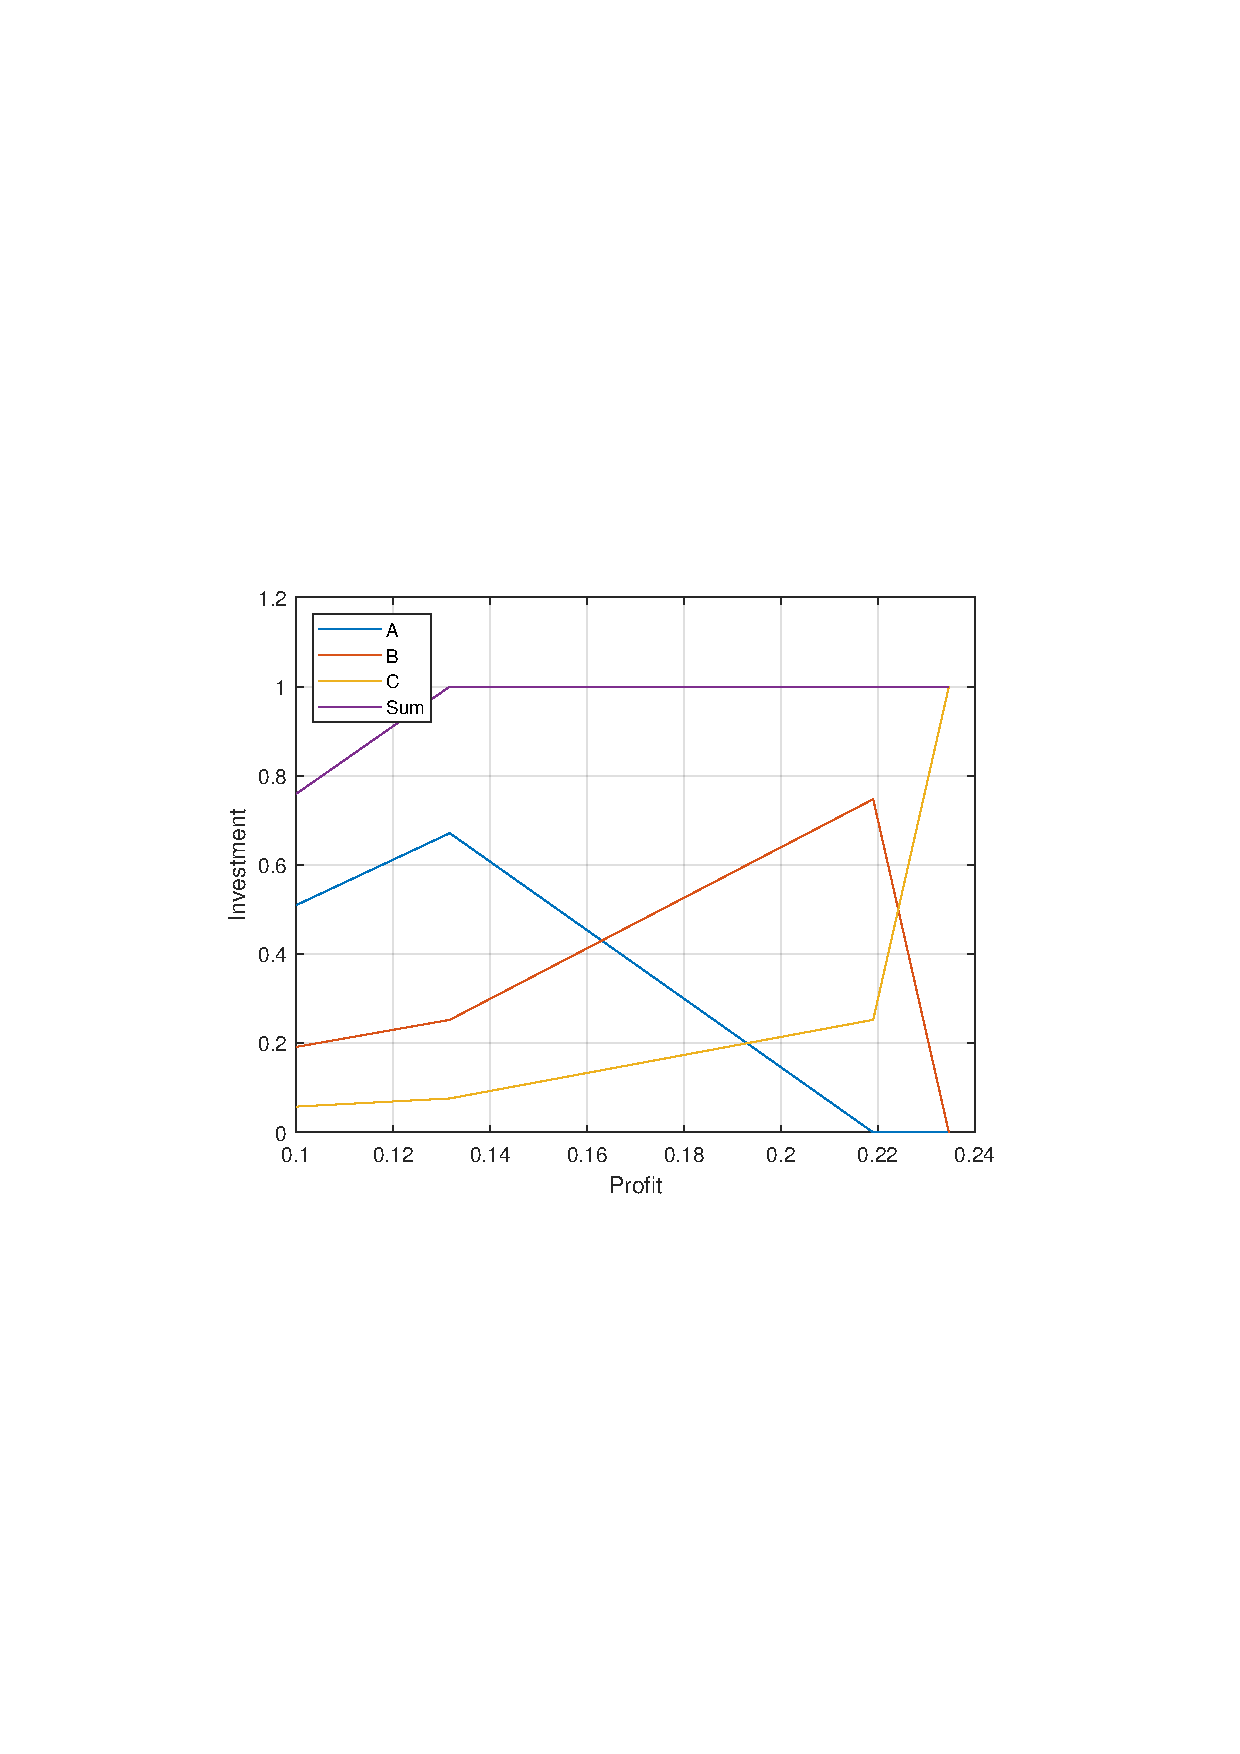
\includegraphics[width=0.8\textwidth,trim={3.09cm 9.295cm 3.09cm 9.295cm},clip]{fig/ex8_invest.pdf}
    \caption{各股投资金额及投资总额占总资金比例随目标收益率的变化曲线}
    \label{fig:ex8_invest}
\end{figure}

\begin{figure}[H]
    \centering
    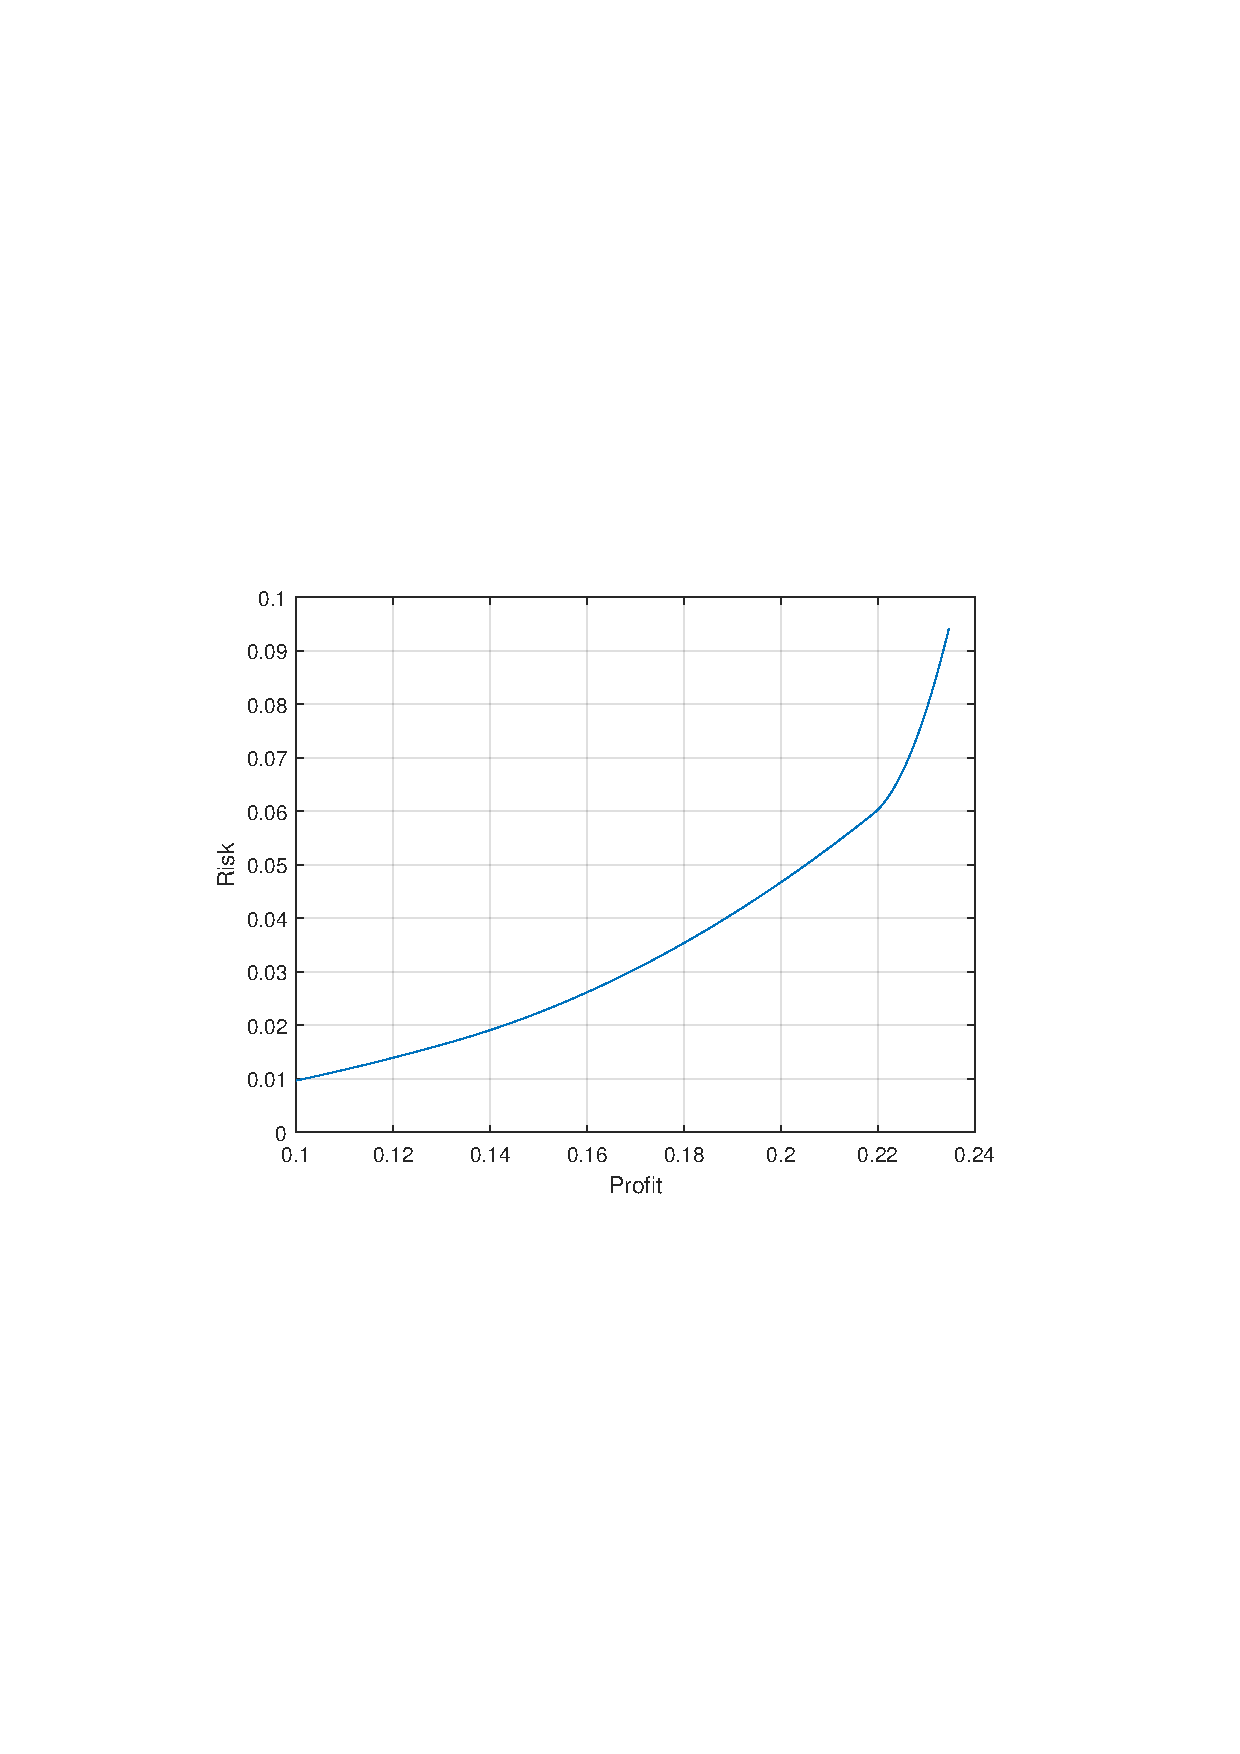
\includegraphics[width=0.8\textwidth,trim={3.09cm 9.295cm 3.09cm 9.295cm},clip]{fig/ex8_risk.pdf}
    \caption{投资风险随目标收益率的变化曲线}
    \label{fig:ex8_risk}
\end{figure}

\paragraph{第(2)问} 假设可以购买年收益率为5\%的无风险国库券,用LINGO求解时,经过94次迭代,找到了全局最优解,风险$f$的最小值为0.0208,各决策变量的最优值如下,所有约束条件(\ref{eq:ex8_cons_range_2}, \ref{eq:ex8_cons_profit})均起约束作用。
\begin{equation}
    \boldsymbol{x} = (0.0870, 0.4282, 0.1435, 0.3412)^T
\end{equation}

用MATLAB求解时,也得到了相同的结果。

\paragraph{第(3)问} 假设目前持有的股票比例为:股票A占50\%,B占35\%,C占15\%,每次股票买卖的交易费为交易额的1\%,用LINGO求解时,经过421次迭代,找到了全局最优解,风险$f$的最小值为0.0226,各决策变量的最优值如下,所有约束条件(\ref{eq:ex8_cons_range_3}, \ref{eq:ex8_cons_profit_3}, \ref{eq:ex8_cons_trans_3})均起约束作用。
\begin{equation}
    \boldsymbol{x} = \left(\begin{matrix}
        0.5266\\
        0.3500\\
        0.1229
    \end{matrix}\right)
    ,\quad
    \boldsymbol{y} = \left(\begin{matrix}
        0.0266\\
        0.0000\\
        0.0000
    \end{matrix}\right)
    ,\quad 
    \boldsymbol{z} = \left(\begin{matrix}
        0.0000\\
        0.0000\\
        0.0271
    \end{matrix}\right)
\end{equation}

\subsubsection{结果的数学分析}

由\Cref{fig:ex8_risk}可以看出,当期望收益越高,相应的风险也越高,体现了高风险高回报的市场规律。由\Cref{fig:ex8_invest}可以看出,当目标收益率较低时,投资者并未将所有的资金投入股市,并倾向于投资低风险低收益的股票A,当目标收益率较高时,投资者将所有资金投入股市,并倾向于投资高风险高收益的股票C。

投资的目标是以最小的风险赚取最大的收益,这是一个多目标优化问题,本题中固定了目标收益率,求最小化风险,实际上也可以在固定的风险承受范围内,求最大的收益,抑或是引入一个平衡因子$\beta$来统一优化收益和风险,即,
\begin{equation}
    \min f = \beta DR - ER
\end{equation}

其中$\beta$越大,表明投资人越厌恶风险。

\subsubsection{结果的实际意义}

在稳定的股票市场中,投资组合模型可作为制定投资策略的重要参考。然而,其局限性也不可忽视,仅仅依靠股票的历史收益序列来估算未来的收益和风险是远远不够的,例如在突如其来的新冠疫情面前,或者瑞幸咖啡的虚假财报面前,该模型将完全失效。

事实上,股票市场往往受到政治经济文化等多方面的影响,除了考虑历史收益,还要考虑公司的运营状况,产业的发展情况,是否有重大利好或利空消息,大盘的走势,广大投资者的心理预期等等,这样才能制定出合适的投资策略。

\subsubsection{结论}

在默认情况下,目标年收益率为15\%,应当以53.02\%的资金投资股票A,35.65的资金投资股票B,11.33\%的资金投资股票C,此时风险最小,为0.0224。

当目标年收益率在10\%-23.46\%之间变化时,投资组合的变化如\Cref{fig:ex8_invest}所示,相应风险的变化如\Cref{fig:ex8_risk}所示,当目标年收益率在23.47\%-100\%之间变化时,没有合适的投资组合。

当可以购买年收益率为5\%的无风险国库券时,应当以8.70\%的资金投资股票A,42.82\%的资金投资股票B,14.35\%的资金投资股票C,34.12\%的资金投资国库券,此时风险最小,为0.0208。

当目前持有的股票比例为:股票A占50\%,B占35\%,C占15\%,每次股票买卖的交易费为交易额的1\%时,应当以2.66\%的资金买入股票A,以2.71\%的资金卖出股票C,持有比例转变为:股票A占52.66\%,B占35.00\%,C占12.29\%,此时风险最小,为0.0226。

\section{收获与建议}

在本次实验中,我掌握了MATLAB优化工具箱和LINGO软件求解线性规划和非线性规划的基本方法,用线性规划和非线性规划方法建立了实际问题的模型,并进行求解,在解决实际问题的过程中,我对数学方法的原理和应用有了更深刻的理解。

希望助教能对每次的实验进行详细的解答,希望老师在未来的课堂上介绍更多数学应用的前沿知识。

\section{附录:程序代码}

\subsection{Chap8-Ex10}\label{sec:ex10_code}

MATLAB程序如下,
\lstinputlisting[language=Matlab]{../src/ex10.m}

LINGO程序如下,
\lstinputlisting[language=Lingo]{../src/ex10.lng}

\subsection{Chap9-Ex4}\label{sec:ex4_code}

MATLAB程序如下,
\lstinputlisting[language=Matlab]{../src/ex4.m}

LINGO程序如下,
\lstinputlisting[language=Lingo]{../src/ex4.lng}

\subsection{Chap9-Ex8}\label{sec:ex8_code}

MATLAB程序如下,
\lstinputlisting[language=Matlab]{../src/ex8.m}

第(0)问和第(1)问的LINGO程序如下,
\lstinputlisting[language=Lingo]{../src/ex8.lng}

第(2)问的LINGO程序如下,
\lstinputlisting[language=Lingo]{../src/ex8_2.lng}

第(3)问的LINGO程序如下,
\lstinputlisting[language=Lingo]{../src/ex8_3.lng}

\end{document}